% !TEX TS-program = pdflatex
% !TEX encoding = UTF-8 Unicode

% This is a simple template for a LaTeX document using the "article" class.
% See "book", "report", "letter" for other types of document.

\documentclass[11pt]{article} % use larger type; default would be 10pt

\usepackage[utf8]{inputenc} % set input encoding (not needed with XeLaTeX)

%%% Examples of Article customizations
% These packages are optional, depending whether you want the features they provide.
% See the LaTeX Companion or other references for full information.

%%% PAGE DIMENSIONS
\usepackage{geometry} % to change the page dimensions
\geometry{a4paper} % or letterpaper (US) or a5paper or....
\geometry{margin=0.5in} 
% \geometry{landscape} % set up the page for landscape
%   read geometry.pdf for detailed page layout information

\usepackage{graphicx} % support the \includegraphics command and options

% \usepackage[parfill]{parskip} % Activate to begin paragraphs with an empty line rather than an indent

%%% PACKAGES
\usepackage{booktabs} % for much better looking tables
\usepackage{array} % for better arrays (eg matrices) in maths
\usepackage{paralist} % very flexible & customisable lists (eg. enumerate/itemize, etc.)
\usepackage{verbatim} % adds environment for commenting out blocks of text & for better verbatim
\usepackage{subfig} % make it possible to include more than one captioned figure/table in a single float
% These packages are all incorporated in the memoir class to one degree or another...

%%% HEADERS & FOOTERS
\usepackage{fancyhdr} % This should be set AFTER setting up the page geometry
\pagestyle{fancy} % options: empty , plain , fancy
\renewcommand{\headrulewidth}{0pt} % customise the layout...
\lhead{}\chead{}\rhead{}
\lfoot{}\cfoot{\thepage}\rfoot{}

%%% SECTION TITLE APPEARANCE
\usepackage{sectsty}
\allsectionsfont{\sffamily\mdseries\upshape} % (See the fntguide.pdf for font help)
% (This matches ConTeXt defaults)

%%% ToC (table of contents) APPEARANCE
\usepackage[nottoc,notlof,notlot]{tocbibind} % Put the bibliography in the ToC
\usepackage[titles,subfigure]{tocloft} % Alter the style of the Table of Contents
\renewcommand{\cftsecfont}{\rmfamily\mdseries\upshape}
\renewcommand{\cftsecpagefont}{\rmfamily\mdseries\upshape} % No bold!

%%% END Article customizations

%%% The "real" document content comes below...

\title{CSU44061 Final Assignment}
\author{17324649 - Efeosa Louis Eguavoen}
%\date{} % Activate to display a given date or no date (if empty),
         % otherwise the current date is printed 

\begin{document}
\maketitle

\section{1}
\subsection{Preprocessing}
The review data we were given was in the form of a JSON in multiple languages.  As the data was in multiple languages and such,  applying machine learning techniques to the data in it's raw for would've proven difficult so some preprocessing was required.  
\\ Initially I considered removing all the removes that were not in English as preprocessing techniques might not work for all the languages in the review data.  I decided against this as just over half of all the reviews in the data were not in English,  and such throwing away that much data would make the final models worse more than likely.  Instead I translated all the non-English reviews to English to get started. 
\begin{verbatim}
def translate_text(text):
    translator = google_translator()
    translation = translator.translate(text)
    origin = text
    translated = translation
    return origin, translated
\end{verbatim}
The above code translates a given review into english and return both the original text and the english version.  I used the Google Translate API to translate into English.
\\ Once the reviews were in English,  I then had to process the data further so it would be in a form that would be usable by the different machine learning techniques I wanted to use.  I started with removing any urls,  emoji's, and numbers from the data.  I also reduced all the words to lower case. 
\begin{verbatim}
def clean_review(review):
    contents = review.lower()
    prepro.set_options(
        prepro.OPT.URL,
        prepro.OPT.EMOJI,
        prepro.OPT.SMILEY,
        prepro.OPT.NUMBER
    )
    clean_contents = prepro.clean(contents)
    contents = clean_contents
    return contents
\end{verbatim}

I then turned the sentences into a list of words or tokens.  I did this so I could then remove all the stop words or words in the english language that don't provide any insight into the meaning of the sentence.  These words occur so frequently also that they don't have any real value hence why I removed them.  Following this,  I lemmatized the tokens.  This process returns a word to it's base.  I chose this over stemming as it's more intelligent as stemming just removes the start or end of a word while lemmatization takes into account the meaning of the word and returns the lemma of it or the dictionary version of the word.
\begin{verbatim}
def tokenize(review):
    tokens = word_tokenize(review)
    stop_words = set(stopwords.words("english"))
    useful_tokens = []
    lemma = WordNetLemmatizer()
    for token in tokens:
        if (not token in stop_words) and (token.isalpha()):
            lemmatnised_token = lemma.lemmatize(token)
            useful_tokens.append(lemmatnised_token)
    return useful_tokens
\end{verbatim}
\subsection{Methods and Hyperparameter Selection}
To see if the review data could 1) Predict the review Polarity and 2) determine if it was in early access or not,  I evaluated 2 very different machine learning models,  A Support Vector Classifier and Convolutional Neural Network.  
\subsubsection{Support Vector Classifier}
A SVC is a supervised machine learning method that tries to find the line that separates the data into it's respective classes,  or the decision boundary.  The main difference between this and Logistic regression is in the loss function, with a SVC using a hinge-loss function.  I went with this method as I wasn't sure if my data was going to be linearly separable as it wasn't numerical data.  SVC's can use non-linear kernels that would adapt better to non-linear data. 
\\ To make the data usable in a SVC  I did a little more preprocessing on the data.  I turned the reviews into a series of vectors using the Term-Frequency and Inverse Document Frequency method or TF-IDF method.  I chose this as using word counts and such was too basic and can be weighted down by words with high frequency and hence lose interesting words in the data.  TF-IDF is better as it prioritises the words in each document so words that occur frequently between documents end up being weighted less as a result of their frequency while words that don't repeat as often are weighted more. 
\begin{verbatim}
def tf_idf(dataset):
    data = dataset["tokens"].values
    tfidf_converter = TfidfVectorizer(min_df=5, max_df=0.7)
    wordDoc = [" ".join(x) for x in data]
    X = tfidf_converter.fit_transform(wordDoc)
    y = dataset["Voted Up"].values
    # df = pd.DataFrame(X[0].T.todense(), index=tfidf_converter.get_feature_names(), columns=["TF-IDF"])
    # df = df.sort_values('TF-IDF', ascending=False)
    # print(df.head())
    return X, y
\end{verbatim}

There are a 3 main hyperparameters to chose for the SVC,  C or how serve a penalty the regulizer gives,  the kernel that's used and Gamma or how muc h influence each point in the data exerts on other points in the dataset. 
\\Given that there's a large number of hyperparameters,  I started with a Gridsearch of the combinations.  I defined a few values of C,  the different kernels I could use and then different Gamma values and evaluated them in terms of Accuracy on the dataset.  This gave me a kind of starting point to tune the data further as I could narrow down the kernel to use.  
\begin{verbatim}
def hyper_pick(X, y):
    """
    Select the best parameters and hyperparameters for the training data using GridSearchCV
    :param X: Tf-IDF scores of tweet data
    :param y:Sentiment values of the tweets
    :return: Outputs a graph of data
    """
    X_train, X_test, y_train, y_test = train_test_split(X, y, test_size=0.2, random_state=101)
    param_grid = [{'C': [0.01, 0.1, 1, 10, 100], 'gamma': [10, 1, 0.1, 0.01, 0.001],
                   'kernel': ['rbf', 'poly', 'sigmoid']}, {'kernel': ['linear'], 'C': [0.01, 0.1, 1, 10, 100],
                                                           'gamma': [10, 1, 0.1, 0.01, 0.001]}]
    grid = GridSearchCV(SVC(), param_grid, refit=True, verbose=2, n_jobs=-1, scoring='accuracy')
    grid.fit(X_train, y_train)
    print(grid.best_params_)
\end{verbatim}
From here I tuned the K and C parameters using 5-fold cross validation.  This outputed a graph so I could then chose an optimal value of K and C. 
\begin{verbatim}
def cross_val(k, model, X, y):
    """
    Inputs: kfold number, machine learning model, data to evaluate X,y

    Outputs: The accuracy, recall and precision and their respective standard deviations for the model
    """
    accuracy_list = []
    recall_list = []
    precision_list = []
    labels = [0, 1]
    kf = KFold(n_splits=k)
    for train, test in kf.split(X):
        model.fit(X[train], y[train])
        predict = model.predict(X[test])

        accuracy = accuracy_score(y[test], predict)
        recall = recall_score(y[test], predict, labels=labels, average='macro')
        precision = precision_score(y[test], predict, labels=labels, average='macro')
        accuracy_list.append(accuracy)
        recall_list.append(recall)
        precision_list.append(precision)

    accuracy_end = np.mean(accuracy_list)
    std = np.std(accuracy_list)
    recall = (np.mean(recall_list), np.std(recall_list))
    precision = (np.mean(precision_list), np.std(precision_list))

    print('Accuracy: ', accuracy_end)
    print('Standard Deviation', std)
    print('Recall', recall)
    print('Precision', precision)

    return accuracy_end, std, recall, precision


def plot_accuracy(X, y):
    """
    Purpose:
        Plots the accuracy and standard deviation for different gamma, C
        Using to fine tune these parameters
    """
    gamma = [0.1, 1, 10, 100]
    C = [0.1, 1, 10, 100]
    plotx = [0, 1, 0, 1]  # lists for plotting
    ploty = [0, 0, 1, 1]  # lists for plotting
    gs = GridSpec(2, 2, wspace=0.3, hspace=0.3)
    fig = plt.figure(figsize=(20,10))
    l = 0
    for i in gamma:

        gx = plotx[l]
        gy = ploty[l]
        ax = fig.add_subplot(gs[gx, gy])
        accuracy_list = []
        std_list = []
        for c in C:
            model = SVC(kernel='sigmoid', gamma=i, C=c)
            accuracy, std, _, _ = cross_val(5, model, X, y)
            accuracy_list.append(accuracy)
            std_list.append(std)
        plt.errorbar(C, accuracy_list, yerr=std_list)
        ax.set_title('Gamma = ' + str(i))
        ax.set_ylabel('Accuracy')
        ax.set_xlabel('C')
        plt.xscale('log')
        l = l + 1
    plt.tight_layout()
    plt.show()
\end{verbatim}
\begin{figure}[h]
\centering
\subfloat[Voted Up]{{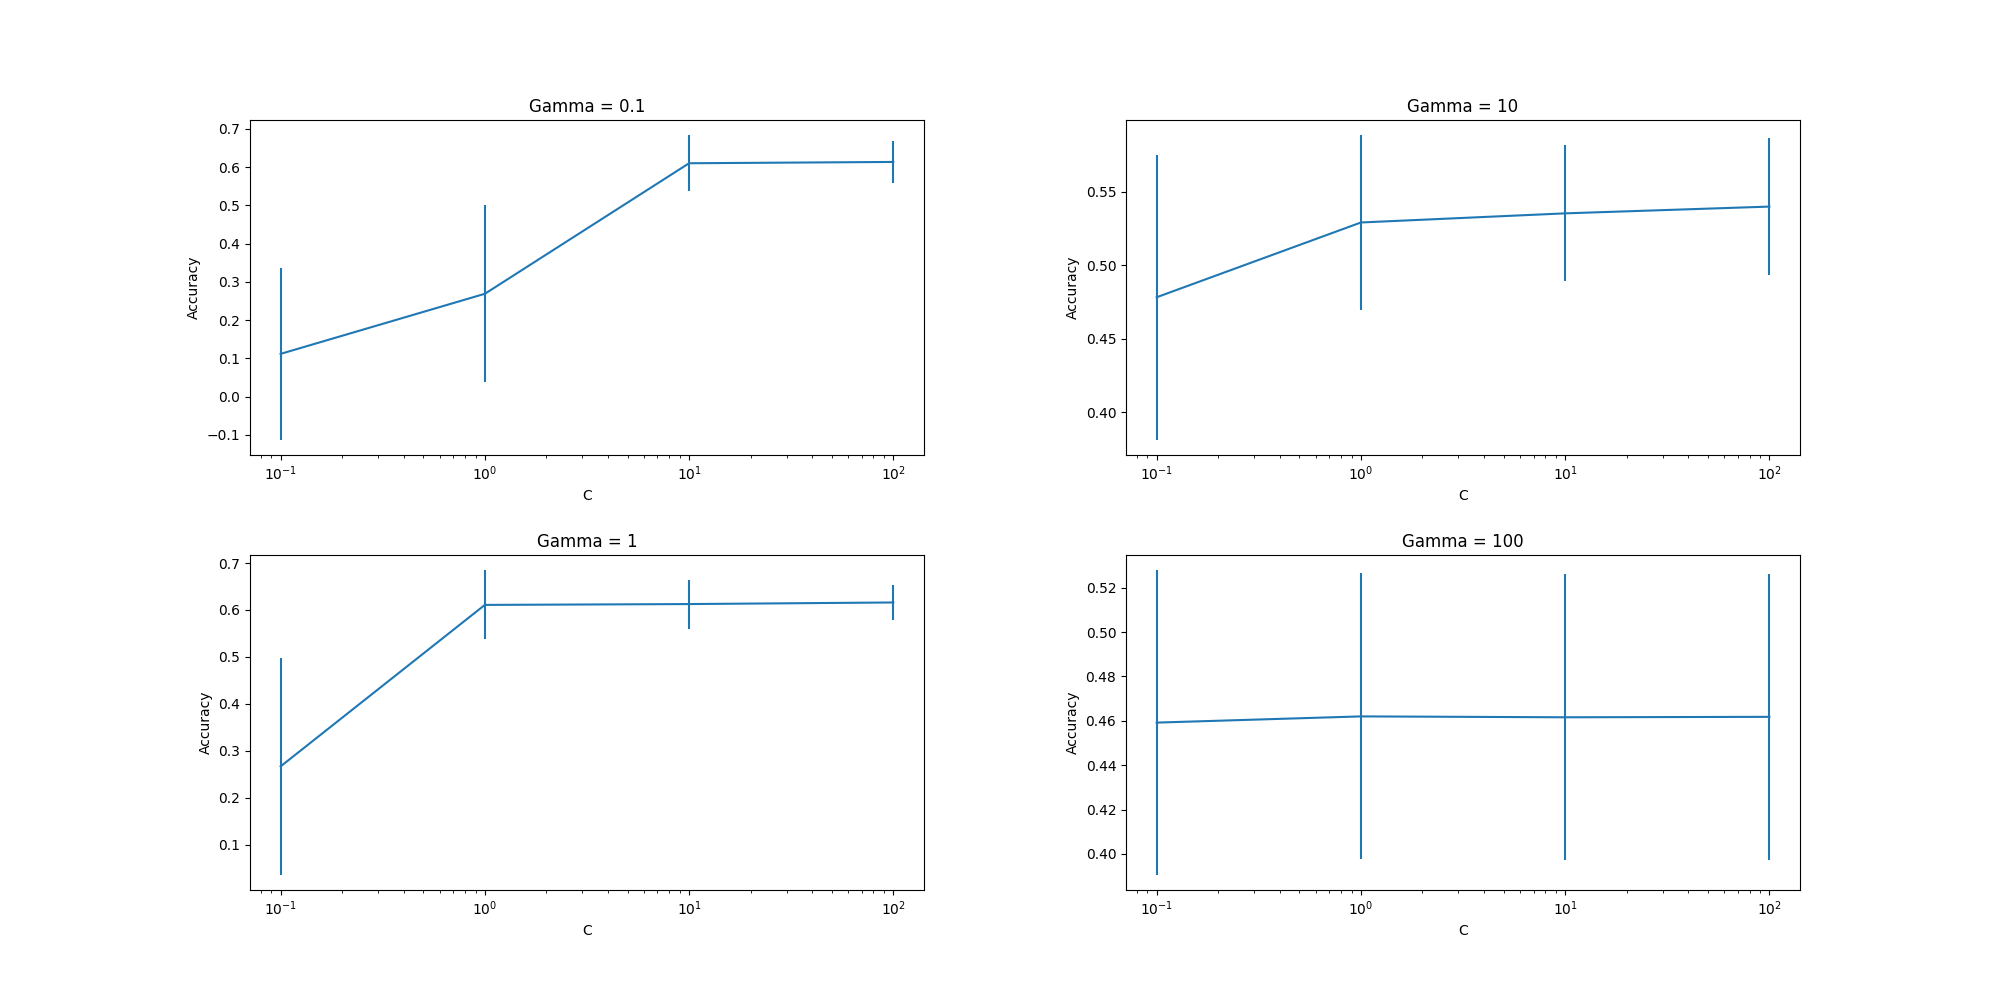
\includegraphics[width=18cm]{myplot.png}}}
\qquad
\subfloat[Early Access]{{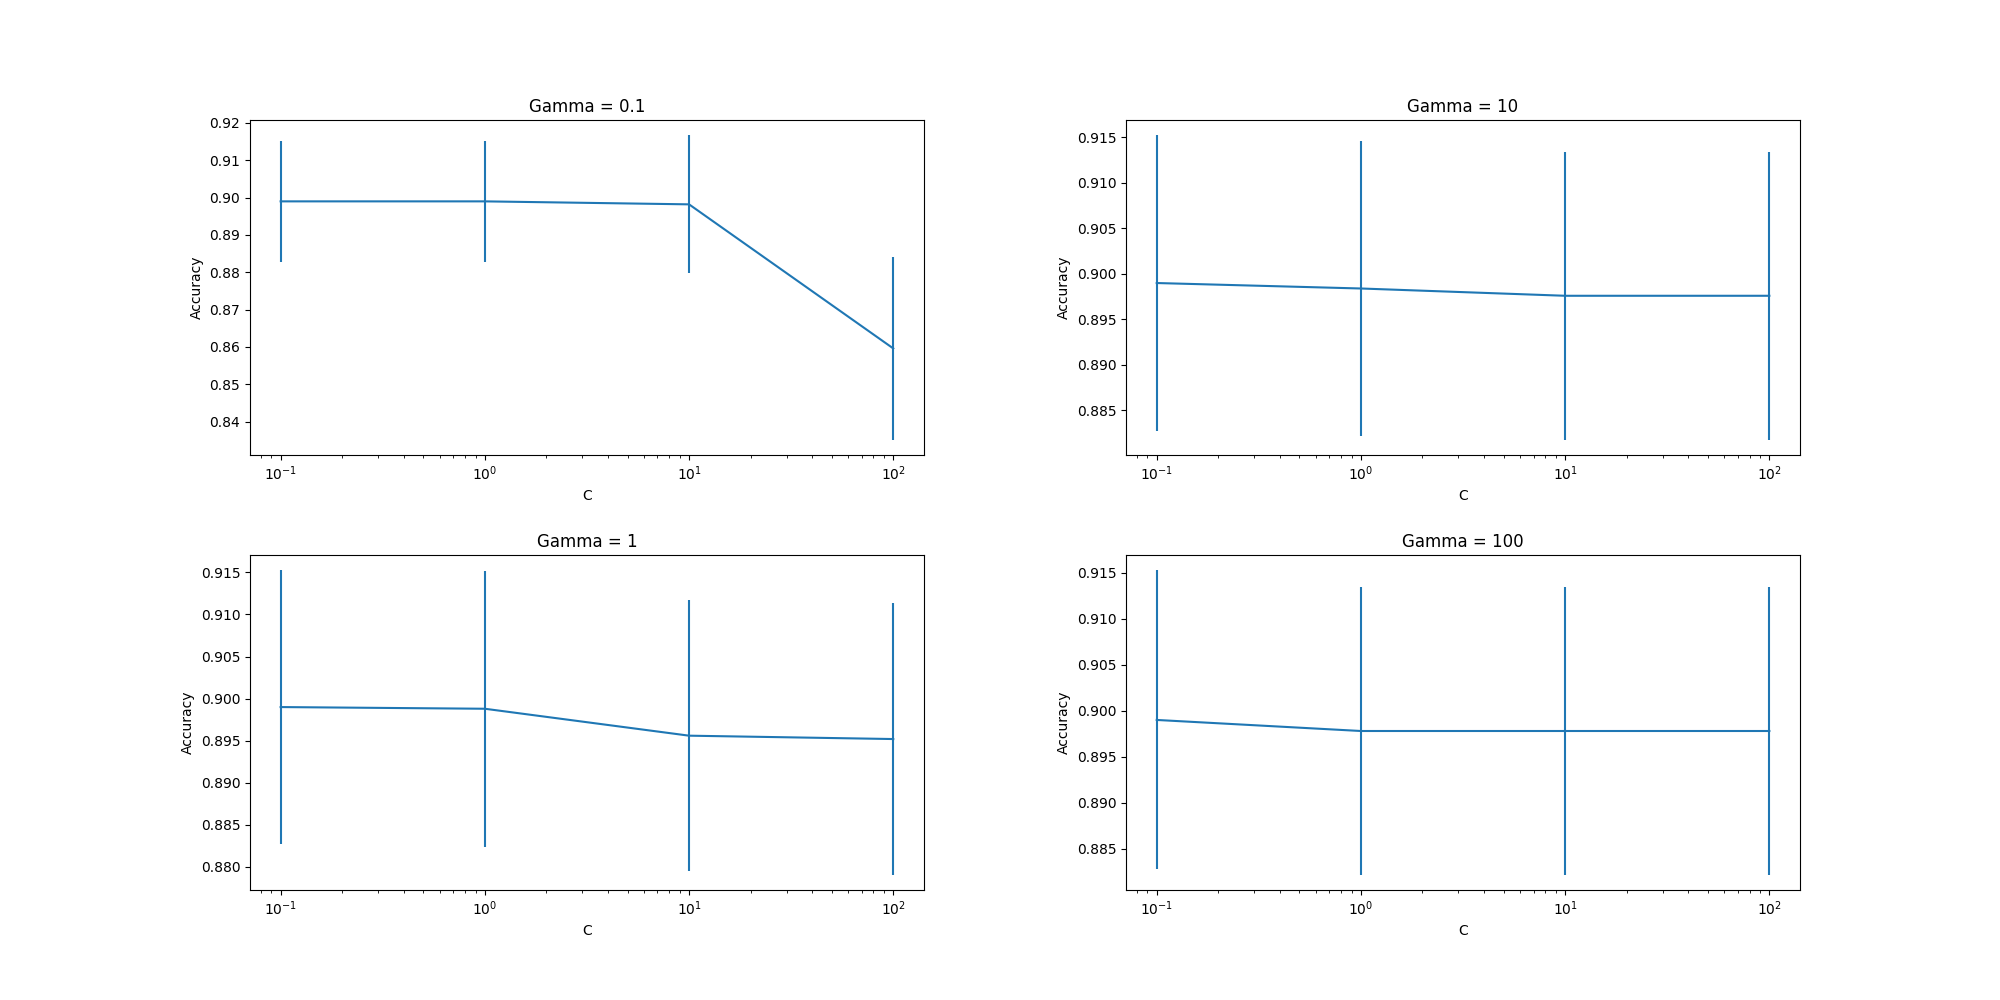
\includegraphics[width=18cm]{eacv.png}}}
\end{figure}

From the above graphs we can see that when C =1 and Gamma = 1 also we can maximise the accuracy so those are the hyper parameters I chose for 'Voted Up'.  From using GridSearchCV,  we found that using a Sigmoid kernel was the best fit for the data. 
\\ For 'Early Access' the graphs indicate that when Gamma = 10 and C = 0.1 with a Gaussian kernel seems to be the best combination of hyper-parameters. 
\subsubsection{Convolutional Neural Network}
For the deep learning algorithms,  I had to go with a different approach for using the text data.  Instead of doing One-Hot Encoding with the TF-IDF vectorizer,  I instead went with a word embedding approach as deep learning needs to know the association between words to make accurate predictions.\\To do this, I made use of the preprocessed texts but used a tokenizer that turned our text corpus into a series of vectors. 
\begin{verbatim}
tokenizer = Tokenizer(num_words=len(TRAINING_VOCAB), lower=True, char_level=False)
    tokenizer.fit_on_texts(train_data["Text_Final"].tolist())
    training_sequences = tokenizer.texts_to_sequences(train_data["Text_Final"].tolist())
\end{verbatim} 
Following this I used Google’s word2vec for word associations since our vocabulary size wasn’t large enough for us to train my own embeddings. For each of our models, I added an embedding layer that acted as our input layer for the vectors.
\begin{verbatim}
train_word_index = tokenizer.word_index
    print('Found %s unique tokens.' % len(train_word_index))
    train_embedding_weights = np.zeros((len(train_word_index) + 1, EMBEDDING_DIM))
    for word, index in train_word_index.items():
        train_embedding_weights[index, :] = word2vec[word] if word in word2vec else np.random.rand(EMBEDDING_DIM)
\end{verbatim}
In terms of hyperparameters,  there's numerous ones to train such as the embedding dimensions size,  the number of convolutional layers we should use,  the batch size we should use for training and numerous others. Tuning all these hyperparameters using cross validation was too time intensive, so instead I focused on cleaning the data better as it provided a more immediate improvement and took much less time to do.  I did attempt to find the optimum amount of Epochs to run the CNN for. 
\begin{figure}[h]
\centering
\subfloat[Voted Up]{{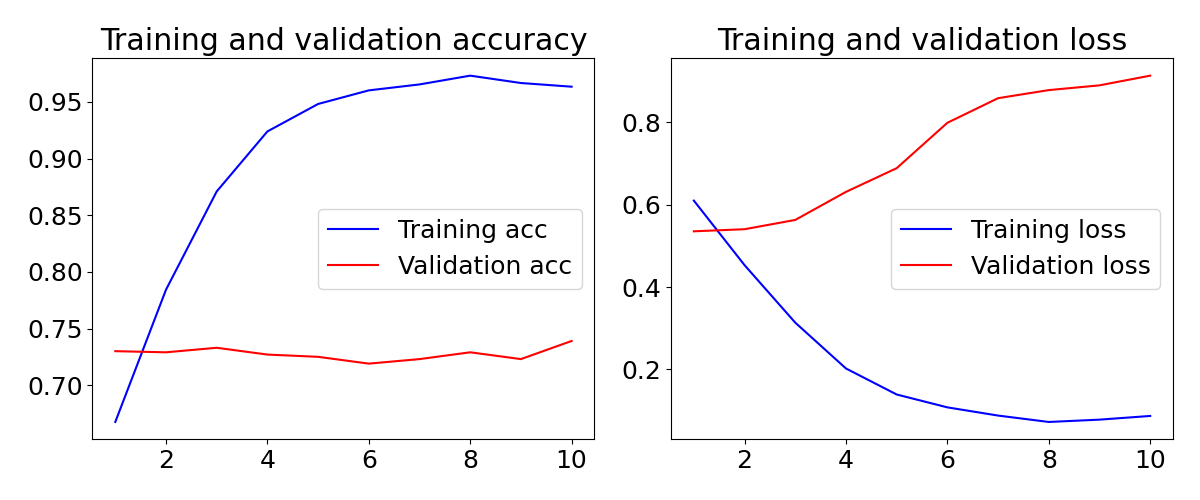
\includegraphics[width=13cm]{vupcnn.png}}}
\qquad
\subfloat[Early Access]{{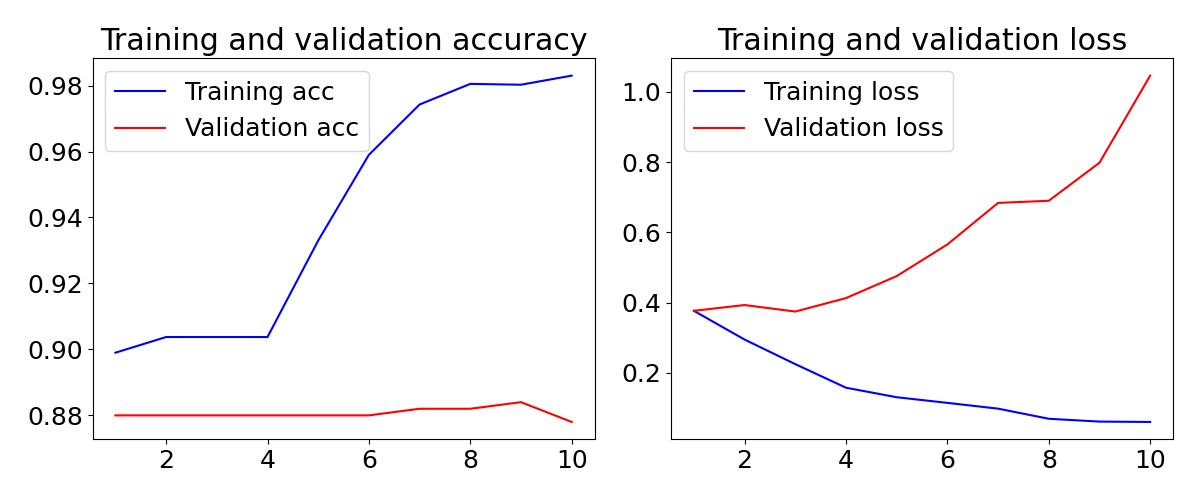
\includegraphics[width=13cm]{eacnn.png}}}
\end{figure}
From the above figures,  training the data for about 3 epochs seems to be the best tradeoff between accuracy and loss for 'Voted Up'
\\ Similarly,  for 'Early Access' it seems about 3 epochs is the sweet spot between accuracy and loss.
\subsection{Results}
To evaluate the results,  I used a baseline that selected the most common class each time and set that as the baseline for performance of the models. I also evaluated the models using a section of the data that I sectioned off before training to act as the test dataset for evaluating the results.
\subsubsection{SVC - Voted Up}
Using the previous hyperparameters with C=1, Gamma =1 and a Sigmoid Kernel we get the following ROC Curve.
\begin{figure}[ht]
\centering
\subfloat[Voted Up]{{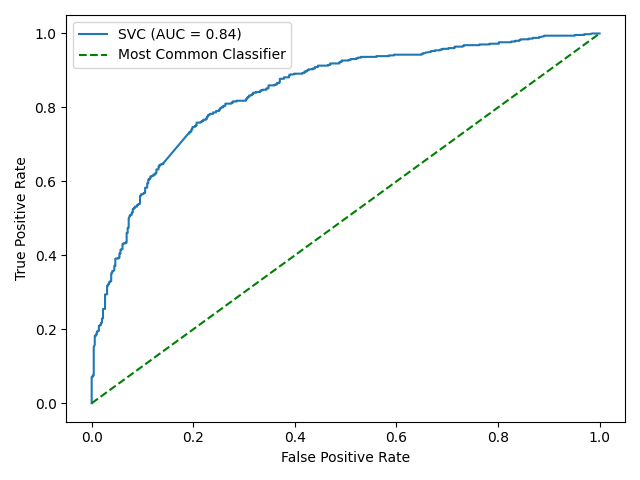
\includegraphics[width=13cm]{rocvup.png}}}
\qquad
\end{figure}
From the curve we can see that our classifier works fairly well.  The total AUC is 0.84 out of a maximum total of 1.  From this we can tell that the classifier is fairly good at distinguishing between the two classes.  The baseline model has an AUC of 0.5 in comparison. 
\\Accuracy : 75\%
\\F1 Score: 77\%
\\ From these above scores, we can see that the model performs well and even beats the baseline model that's only correct around 50\% of the time due to the fact the data is split 50/50 in terms of being voted up or not.
\subsubsection{CNN - Voted Up}
Accuracy:  73\%
\\ F1 Score: 73\%
\\ From the above figures we can see that for the CNN, it's accuracy is comparable to the SVC, in terms of getting the polarity of the review(Voted Up or not). The F1 Score is also comparable.
\newpage
\subsubsection{SVC - Early Access}
Using the previous hyperparameters selected, we get the below ROC Curve. From the curve we can tell that the classifier isn't able to distinguish between the classes very well at. The roc curve is almost exactly a diagonal line, reinforcing this.
\begin{figure}[ht]
\centering
\subfloat[Voted Up]{{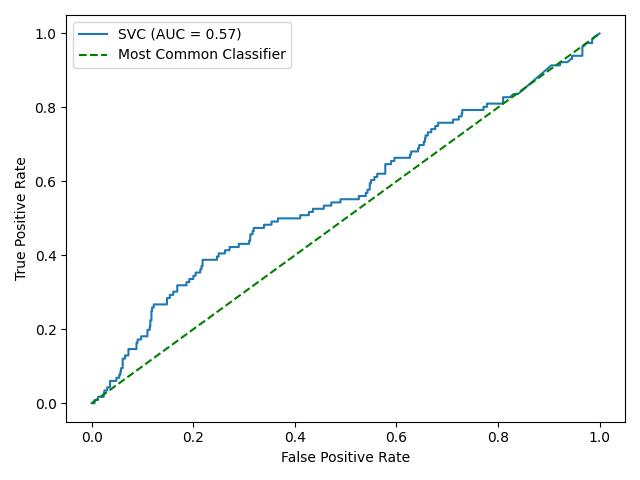
\includegraphics[width=13cm]{earoc.png}}}
\qquad
\end{figure}
\\F1 Score:  .4714587737843552
\\Precision Score:  0.446
\\Accuracy Score:  89\%
\\ From the above figures, we can see the accuracy of the SVC classifier is high, but in comparison, the baseline model that picks the most common class has the exact same level of accuracy(89\%). But the F1 and Precision score are very low or in other words the model is predicting the most common class but almost never capturing the class that's not so common.
\subsubsection{CNN - Early Access}
Accuracy:  90\%
\\ F1 Score: 0.896
\\Precision: 0.898
\\ From the above figures we can see Accuracy of the CNN classifier works just as well as the SVC classifier and the baseline model. But in comparison to both these classifiers, the CNN is much better at differenciating between the classes, as seen by the high F1 Score. The SVC wasn't able to differenciate between the classes very well but the CNN can both differenciate between the classes and also maintain high accuracy also which is great as class that occurs less often still gets identified when it does occur. 

\subsection{Conclusions}
From the results, we can see that both classifiers are good at predicting the polarity of reviews, with them both performing better than the baseline model. The precision and recall of these models is sufficently high that they can distinguish between the classes well also.
\\ In comparison though, when detecting if a review is in early access, the SVC classifier isn't as good at detecting if the review is for an early access game due to the low F1 and Precision score. But the CNN can both differenciate between the classes and maintain a high level of Accuracy which is a very important as otherwise, the model wouldn't be any better than just predicting the most common class.
\subsection{Code Appendix}
\subsubsection{FinalAssignment.py}
\begin{verbatim}
import json
import re
from os import path
import pandas as pd
from google_trans_new import google_translator
from FinalAssignment.svc_classifier import main as svc
from FinalAssignment.CNN import main as cnn
from FinalAssignment.pre_proceess import main as pre_process


def read_file(text=None):
    if text is None:
        Y = []
        Z = []
        with open('reviews_262.jl.txt', encoding='utf8') as json_file:
            text_vals = []
            for i in json_file:
                data = json.loads(i)
                text_vals.append(data['text'])
                Y.append(data['voted_up'])
                Z.append(data['early_access'])
            return text_vals, Y, Z
    translations = []
    with open(text, encoding='utf-8') as json_file:
        for i in json_file:
            data = json.loads(i)
            try:
                translations.append(data['text'])
            except TypeError:
                return pd.DataFrame(json.loads(i))
    return translations


def fixFile():
    with open('translations.txt', 'r', encoding="utf-8") as s:
        with open('new_translations.txt', 'a', encoding="utf-8") as f:
            for i in s:
                matches = re.findall(r'\"(.+?)\"', i)
                matches.pop(0)
                f.write('{"text" : ' + '"' + ",".join(matches) + '"' + '}' + '\n')


def translate_text(text):
    translator = google_translator()
    translation = translator.translate(text)
    origin = text
    translated = translation
    return origin, translated


def write_translations(texts):
    with open('translations.txt', 'a', encoding="utf-8") as f:
        for text in texts:
            f.write('{"text" : ' + '"' + text + '"' + '}' + '\n')


def main():
    texts, Y, Z = read_file()
    translated = []
    if path.exists('new_translations.txt'):
        # fixFile()
        translated = read_file('new_translations.txt')
    else:
        i = 0
        for text in texts:
            if i >= 4643:
                part_origin, part_translated = translate_text(text)
                translated.append(part_translated)
                write_translations(translated)
                translated = []
            i = i + 1
    dataset = pd.DataFrame({'Text': translated,
                            'Voted Up': Y,
                            'Early Access': Z})
    if not path.exists('processed_reviews.txt'):
        pre_process(dataset['Text'])
    else:
        tokens = read_file('processed_reviews.txt')
        dataset["tokens"] = tokens
    print(dataset.loc[0])
    # svc(dataset)
    print(dataset.groupby('Early Access').count())
    cnn(dataset)


if __name__ == '__main__':
    main()
\end{verbatim}
\subsubsection{pre\_procces.py}
\begin{verbatim}
import nltk
from nltk.corpus import stopwords
from nltk.tokenize import word_tokenize
from nltk.stem import WordNetLemmatizer
import preprocessor as prepro
import json
from os import path


def clean_review(review):
    contents = review.lower()
    # May want to change these
    prepro.set_options(
        prepro.OPT.URL,
        prepro.OPT.EMOJI,
        prepro.OPT.SMILEY,
        prepro.OPT.NUMBER
    )
    clean_contents = prepro.clean(contents)
    contents = clean_contents
    return contents


def tokenize(review):
    tokens = word_tokenize(review)
    stop_words = set(stopwords.words("english"))
    useful_tokens = []
    lemma = WordNetLemmatizer()
    for token in tokens:
        if (not token in stop_words) and (token.isalpha()):
            lemmatnised_token = lemma.lemmatize(token)
            useful_tokens.append(lemmatnised_token)
    return useful_tokens


def main(reviews):
    # nltk.download()
    processed_reviews = []
    for review in reviews:
        review = clean_review(review)
        tokens = tokenize(review)
        processed_reviews.append({"tokens": tokens})
    with open("processed_reviews.txt", "w") as f:
        f.write(json.dumps(processed_reviews))
\end{verbatim}
\subsection{svc\_classifier.py}
\begin{verbatim}
def tf_idf(dataset):
    """
    Gets the TF-IDF scores for the tweets in the dataframe to be used for Other Machine Learning Algorithms
    :param dataset: Dataframe containing preprocessed tweets
    :return: X: Scores, Y:Sentiment values
    """
    data = dataset["tokens"].values
    tfidf_converter = TfidfVectorizer(min_df=5, max_df=0.7)
    wordDoc = [" ".join(x) for x in data]
    X = tfidf_converter.fit_transform(wordDoc)
    y = dataset["Early Access"].values
    # df = pd.DataFrame(X[0].T.todense(), index=tfidf_converter.get_feature_names(), columns=["TF-IDF"])
    # df = df.sort_values('TF-IDF', ascending=False)
    # print(df.head())
    return X, y


def hyper_pick(X, y):
    """
    Select the best parameters and hyperparameters for the training data using GridSearchCV
    :param X: Tf-IDF scores of tweet data
    :param y:Sentiment values of the tweets
    :return: Outputs a graph of data
    """
    X_train, X_test, y_train, y_test = train_test_split(X, y, test_size=0.2, random_state=101)
    param_grid = [{'C': [0.01, 0.1, 1, 10, 100], 'gamma': [10, 1, 0.1, 0.01, 0.001],
                   'kernel': ['rbf', 'poly', 'sigmoid']}, {'kernel': ['linear'], 'C': [0.01, 0.1, 1, 10, 100],
                                                           'gamma': [10, 1, 0.1, 0.01, 0.001]}]
    grid = GridSearchCV(SVC(), param_grid, refit=True, verbose=2, n_jobs=-1, scoring='accuracy')
    grid.fit(X_train, y_train)
    print(grid.best_params_)


def svm(X, y):
    """
    Trains SVM Classifier
    :param X: TF-IDF Scores
    :param y:
    :return:
    """
    labels = [0, 1]
    X_train, X_test, y_train, y_test = train_test_split(X, y, test_size=0.2)
    clf = SVC(kernel='rbf', gamma=10, C=0.01)
    clf.fit(X_train, y_train)
    predict = clf.predict(X_test)
    print('Confusion Matrix: ', confusion_matrix(y_test, predict, labels=labels))
    print('F1 Score: ', f1_score(y_test, predict, labels=labels, average='macro'))
    print('Precision Score: ', precision_score(y_test, predict, labels=labels, average='macro'))
    print('Accuracy Score: ', accuracy_score(y_test, predict))
    plot_roc_curve(clf,X_test,y_test)
    plt.show()
    print(classification_report(y_test, predict, digits=3))
    print('Recall: ', recall_score(y_test, predict, labels=labels, average='macro'))



def cross_val(k, model, X, y):
    """
    Inputs: kfold number, machine learning model, data to evaluate X,y

    Outputs: The accuracy, recall and precision and their respective standard deviations for the model
    """
    accuracy_list = []
    recall_list = []
    precision_list = []
    labels = [0, 1]
    kf = KFold(n_splits=k)
    for train, test in kf.split(X):
        model.fit(X[train], y[train])
        predict = model.predict(X[test])

        accuracy = accuracy_score(y[test], predict)
        recall = recall_score(y[test], predict, labels=labels, average='macro')
        precision = precision_score(y[test], predict, labels=labels, average='macro')
        accuracy_list.append(accuracy)
        recall_list.append(recall)
        precision_list.append(precision)

    accuracy_end = np.mean(accuracy_list)
    std = np.std(accuracy_list)
    recall = (np.mean(recall_list), np.std(recall_list))
    precision = (np.mean(precision_list), np.std(precision_list))

    print('Accuracy: ', accuracy_end)
    print('Standard Deviation', std)
    print('Recall', recall)
    print('Precision', precision)

    return accuracy_end, std, recall, precision


def plot_accuracy(X, y):
    """
    Purpose:
        Plots the accuracy and standard deviation for different gamma, C
        Using to fine tune these parameters
    """
    gamma = [0.1, 1, 10, 100]
    C = [0.1, 1, 10, 100]
    plotx = [0, 1, 0, 1]  # lists for plotting
    ploty = [0, 0, 1, 1]  # lists for plotting
    gs = GridSpec(2, 2, wspace=0.3, hspace=0.3)
    fig = plt.figure(figsize=(20,10))
    l = 0
    for i in gamma:

        gx = plotx[l]
        gy = ploty[l]
        ax = fig.add_subplot(gs[gx, gy])
        accuracy_list = []
        std_list = []
        for c in C:
            model = SVC(kernel='rbf', gamma=i, C=c)
            accuracy, std, _, _ = cross_val(5, model, X, y)
            accuracy_list.append(accuracy)
            std_list.append(std)
        plt.errorbar(C, accuracy_list, yerr=std_list)
        ax.set_title('Gamma = ' + str(i))
        ax.set_ylabel('Accuracy')
        ax.set_xlabel('C')
        plt.xscale('log')
        l = l + 1
    plt.tight_layout()
    plt.show()


def main(review_dataset):
    X, y = tf_idf(review_dataset)
    # hyper_pick(X, y)
    svm(X, y)
    # cross_val(5, SVC(kernel='rbf', gamma=1, C=100), X, y)
    # plot_accuracy(X,y)
\end{verbatim}
\subsection{CNN.py}
\begin{verbatim}
ef plot_history(history):
    acc = history.history['acc']
    val_acc = history.history['val_acc']
    loss = history.history['loss']
    val_loss = history.history['val_loss']
    x = range(1, len(acc) + 1)
    plt.rc('font', size=18)
    plt.clf()
    plt.figure(figsize=(12, 5))
    plt.subplot(1, 2, 1)
    plt.plot(x, acc, 'b', label='Training acc')
    plt.plot(x, val_acc, 'r', label='Validation acc')
    plt.title('Training and validation accuracy')
    plt.legend()
    plt.subplot(1, 2, 2)
    plt.plot(x, loss, 'b', label='Training loss')
    plt.plot(x, val_loss, 'r', label='Validation loss')
    plt.title('Training and validation loss')
    plt.legend()
    plt.show()


def reprocess_data(dataset):
    dataset['Text_Final'] = [' '.join(x) for x in dataset['tokens']]
    pos = []
    neg = []
    for l in dataset['Early Access']:
        if l == 1:
            pos.append(1)
            neg.append(0)
        elif l == 0:
            pos.append(0)
            neg.append(1)

    dataset['Pos'] = pos
    dataset['Neg'] = neg


def test_train_split(dataset):
    train_data, test_data = train_test_split(dataset, test_size=0.2)
    all_training_words = [word for tokens in train_data["tokens"] for word in tokens]
    training_sentence_lengths = [len(tokens) for tokens in train_data["tokens"]]
    TRAINING_VOCAB = sorted(list(set(all_training_words)))
    print("%s words total, with a vocabulary size of %s" % (len(all_training_words), len(TRAINING_VOCAB)))
    print("Max sentence length is %s" % max(training_sentence_lengths))

    all_test_words = [word for tokens in test_data["tokens"] for word in tokens]
    test_sentence_lengths = [len(tokens) for tokens in test_data["tokens"]]
    TEST_VOCAB = sorted(list(set(all_test_words)))
    print("%s words total, with a vocabulary size of %s" % (len(all_test_words), len(TEST_VOCAB)))
    print("Max sentence length is %s" % max(test_sentence_lengths))

    return train_data, test_data, TRAINING_VOCAB, TEST_VOCAB


def get_average_word2vec(tokens_list, vector, generate_missing=False, k=300):
    if len(tokens_list) < 1:
        return np.zeros(k)
    if generate_missing:
        vectorized = [vector[word] if word in vector else np.random.rand(k) for word in tokens_list]
    else:
        vectorized = [vector[word] if word in vector else np.zeros(k) for word in tokens_list]
    length = len(vectorized)
    summed = np.sum(vectorized, axis=0)
    averaged = np.divide(summed, length)
    return averaged


def get_word2vec_embeddings(vectors, clean_comments, generate_missing=False):
    embeddings = clean_comments['tokens'].apply(lambda x: get_average_word2vec(x, vectors,
                                                                               generate_missing=generate_missing))
    return list(embeddings)


def ConvNet(embeddings, max_sequence_length, num_words, embedding_dim, labels_index):
    embedding_layer = Embedding(num_words, embedding_dim, weights=[embeddings], input_length=max_sequence_length,
                                trainable=False)

    sequence_input = Input(shape=(max_sequence_length,), dtype='int32')
    embedded_sequences = embedding_layer(sequence_input)

    convs = []
    filter_sizes = [2, 3, 4, 5, 6]
    for filter_size in filter_sizes:
        l_conv = Conv1D(filters=200, kernel_size=filter_size, activation='relu')(embedded_sequences)
        l_pool = GlobalMaxPooling1D()(l_conv)
        convs.append(l_pool)

    l_merge = concatenate(convs, axis=1)

    x = Dropout(0.1)(l_merge)
    x = Dense(128, activation='relu')(x)
    x = Dropout(0.2)(x)
    preds = Dense(labels_index, activation='sigmoid')(x)

    model = Model(sequence_input, preds)
    model.compile(loss='binary_crossentropy',
                  optimizer='adam',
                  metrics=['acc'])
    model.summary()
    return model


def recall_m(y_true, y_pred):
    true_positives = K.sum(K.round(K.clip(y_true * y_pred, 0, 1)))
    possible_positives = K.sum(K.round(K.clip(y_true, 0, 1)))
    recall = true_positives / (possible_positives + K.epsilon())
    return recall


def precision_m(y_true, y_pred):
    true_positives = K.sum(K.round(K.clip(y_true * y_pred, 0, 1)))
    predicted_positives = K.sum(K.round(K.clip(y_pred, 0, 1)))
    precision = true_positives / (predicted_positives + K.epsilon())
    return precision


def f1_m(y_true, y_pred):
    precision = precision_m(y_true, y_pred)
    recall = recall_m(y_true, y_pred)
    return 2 * ((precision * recall) / (precision + recall + K.epsilon()))


def cross_val_NN(k, X, y, train_embedding_weights, MAX_SEQUENCE_LENGTH,
                 train_word_index, EMBEDDING_DIM, label_names, max_epoch,
                 nnmodel):
    """
    Inputs: kfold number, data to evaluate X,y and setting for the model

    Outputs: The accuracy, precision, recall and standard deviation of the model
    """

    accuracy_list = []
    recall_list = []
    precision_list = []
    kf = KFold(n_splits=k)
    model = None

    for train, test in kf.split(X, y):
        if nnmodel == 'CNN':
            model = ConvNet(train_embedding_weights, MAX_SEQUENCE_LENGTH, len(train_word_index) + 1, EMBEDDING_DIM,
                            len(list(label_names)))
        model.compile(optimizer='adam', loss='binary_crossentropy', metrics=['acc', f1_m, precision_m, recall_m])

        model.fit(X[train], y[train], epochs=max_epoch, batch_size=34, validation_data=(X[test], y[test]))
        # predict=model.predict(X[test])
        loss, accuracy, f1_score, precision, recall = model.evaluate(X[test], y[test], verbose=0)

        accuracy_list.append(accuracy)
        recall_list.append(recall)
        precision_list.append(precision)

    accuracy_end = np.mean(accuracy_list)
    std = np.std(accuracy_list)
    recall = (np.mean(recall_list), np.std(recall_list))
    precision = (np.mean(precision_list), np.std(precision_list))

    print('Accuracy: ', accuracy_end)
    print('Standard Deviation', std)
    print('Recall', recall)
    print('Precision', precision)

    return accuracy_end, std, recall, precision

def main(reviews):
    reprocess_data(reviews)
    train_data, test_data, TRAINING_VOCAB, TEST_VOCAB = test_train_split(reviews)
    word2vec_path = 'GoogleNews-vectors-negative300.bin.gz'
    word2vec = models.KeyedVectors.load_word2vec_format(word2vec_path, binary=True)
    training_embeddings = get_word2vec_embeddings(word2vec, train_data, generate_missing=True)
    MAX_SEQUENCE_LENGTH = 50
    EMBEDDING_DIM = 300
    tokenizer = Tokenizer(num_words=len(TRAINING_VOCAB), lower=True, char_level=False)
    tokenizer.fit_on_texts(train_data["Text_Final"].tolist())
    training_sequences = tokenizer.texts_to_sequences(train_data["Text_Final"].tolist())

    train_word_index = tokenizer.word_index
    print('Found %s unique tokens.' % len(train_word_index))
    train_embedding_weights = np.zeros((len(train_word_index) + 1, EMBEDDING_DIM))
    for word, index in train_word_index.items():
        train_embedding_weights[index, :] = word2vec[word] if word in word2vec else np.random.rand(EMBEDDING_DIM)

    train_cnn_data = pad_sequences(training_sequences, maxlen=MAX_SEQUENCE_LENGTH)
    test_sequences = tokenizer.texts_to_sequences(test_data["Text_Final"].tolist())
    test_cnn_data = pad_sequences(test_sequences, maxlen=MAX_SEQUENCE_LENGTH)
    label_names = ['Pos', 'Neg']
    y_train = train_data[label_names].values
    y_test = test_data[label_names].values
    x_train = train_cnn_data
    x_test = test_cnn_data
    model = ConvNet(train_embedding_weights, MAX_SEQUENCE_LENGTH, len(train_word_index) + 1, EMBEDDING_DIM,
    len(list(label_names)))
    history = model.fit(x_train, y_train, epochs=3, batch_size=64, validation_data=(x_test, y_test))
    # plot_history(history)
    X=np.concatenate((x_train,x_test))
    y=np.concatenate((y_train,y_test))
    cross_val_NN(5,X,y,train_embedding_weights,MAX_SEQUENCE_LENGTH,
                 train_word_index,EMBEDDING_DIM,label_names,max_epoch=5,
                 nnmodel='CNN')
\end{verbatim}
\section{2}
\end{document}
